\documentclass[12pt, letterpaper]{article}
\usepackage[utf8]{inputenc}
\usepackage[margin=1in]{geometry}
\usepackage[super]{nth}
\usepackage{hyperref}
\usepackage{lineno}
\usepackage[
singlelinecheck=false
]{caption}
\usepackage{amsmath}
\usepackage{amsfonts}
\usepackage{bm}
\usepackage{bbm}
\usepackage{graphicx}
\usepackage{csvsimple}
\usepackage[section]{placeins}
\usepackage{lineno}
\usepackage{natbib}

\title{A joint framework for the estimation of PCA and F-statistics using ancient DNA}
\author{Divyaratan Popli, Benjamin M. Peter}
%\date{5 August 2021}
\linenumbers

\setlength{\parskip}{1em}
\setlength{\parindent}{0em}

\newcommand{\BZ}{\mathbf{Z}}
\newcommand{\BD}{\mathbf{D}}
\newcommand{\BN}{\mathbf{N}}
\newcommand{\BH}{\mathbf{H}}
\newcommand{\Btheta}{\pmb{\theta}}


\begin{document}

\maketitle
%\renewcommand\thefigure{\arabic{figure}}    
\section*{Supplementary Figures}
%\setcounter{figure}{0}   
\renewcommand{\figurename}{Fig S}


\begin{figure}[ht!]
    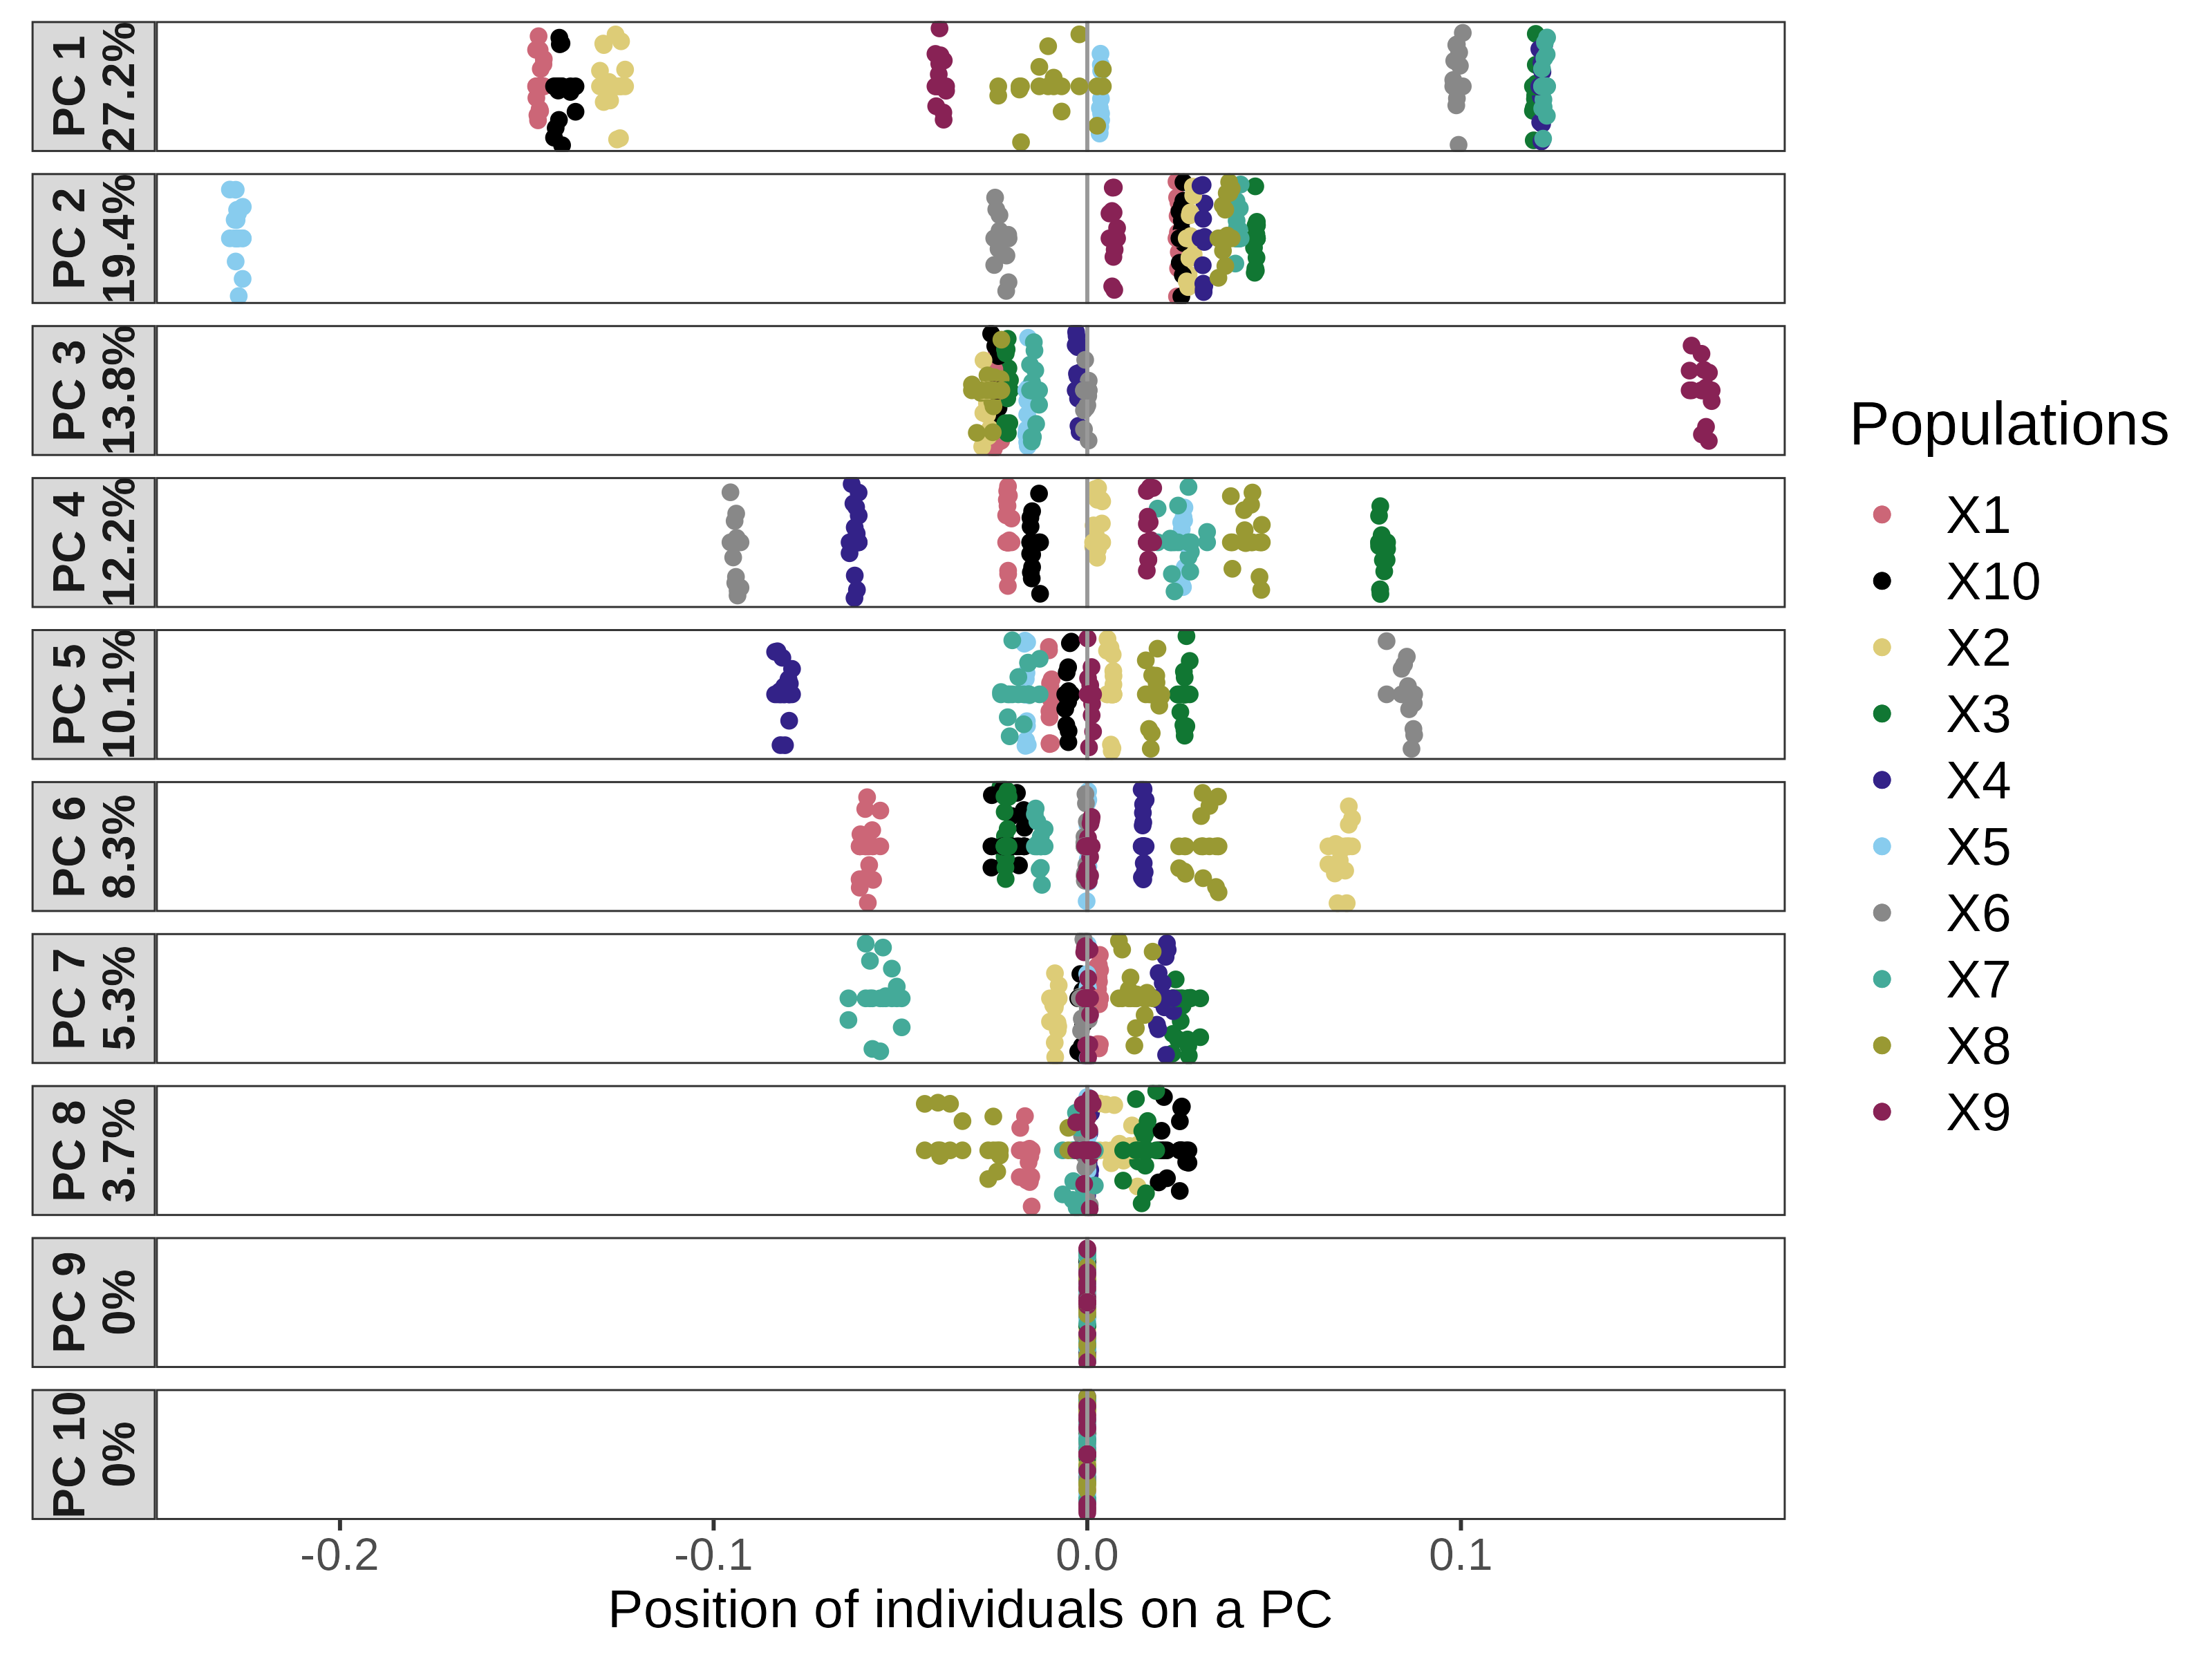
\includegraphics[width=16.5cm]{Images/Supplement/pcplot2.png}
    \centering
    \caption{Variation in the genetic data explained with the top 10 PCs from PPCA. Each panel shows the position of individuals on a Principal Component. Jitter is added to y-axis to show the data points clearly. The last 2 PCs explain $0\%$ variation because the PPCA model with scale=8 explicitly sets the non- relevant PCs to 0.}
    \label{figS1:pc_scale}
\end{figure}

\begin{figure}[ht!]
    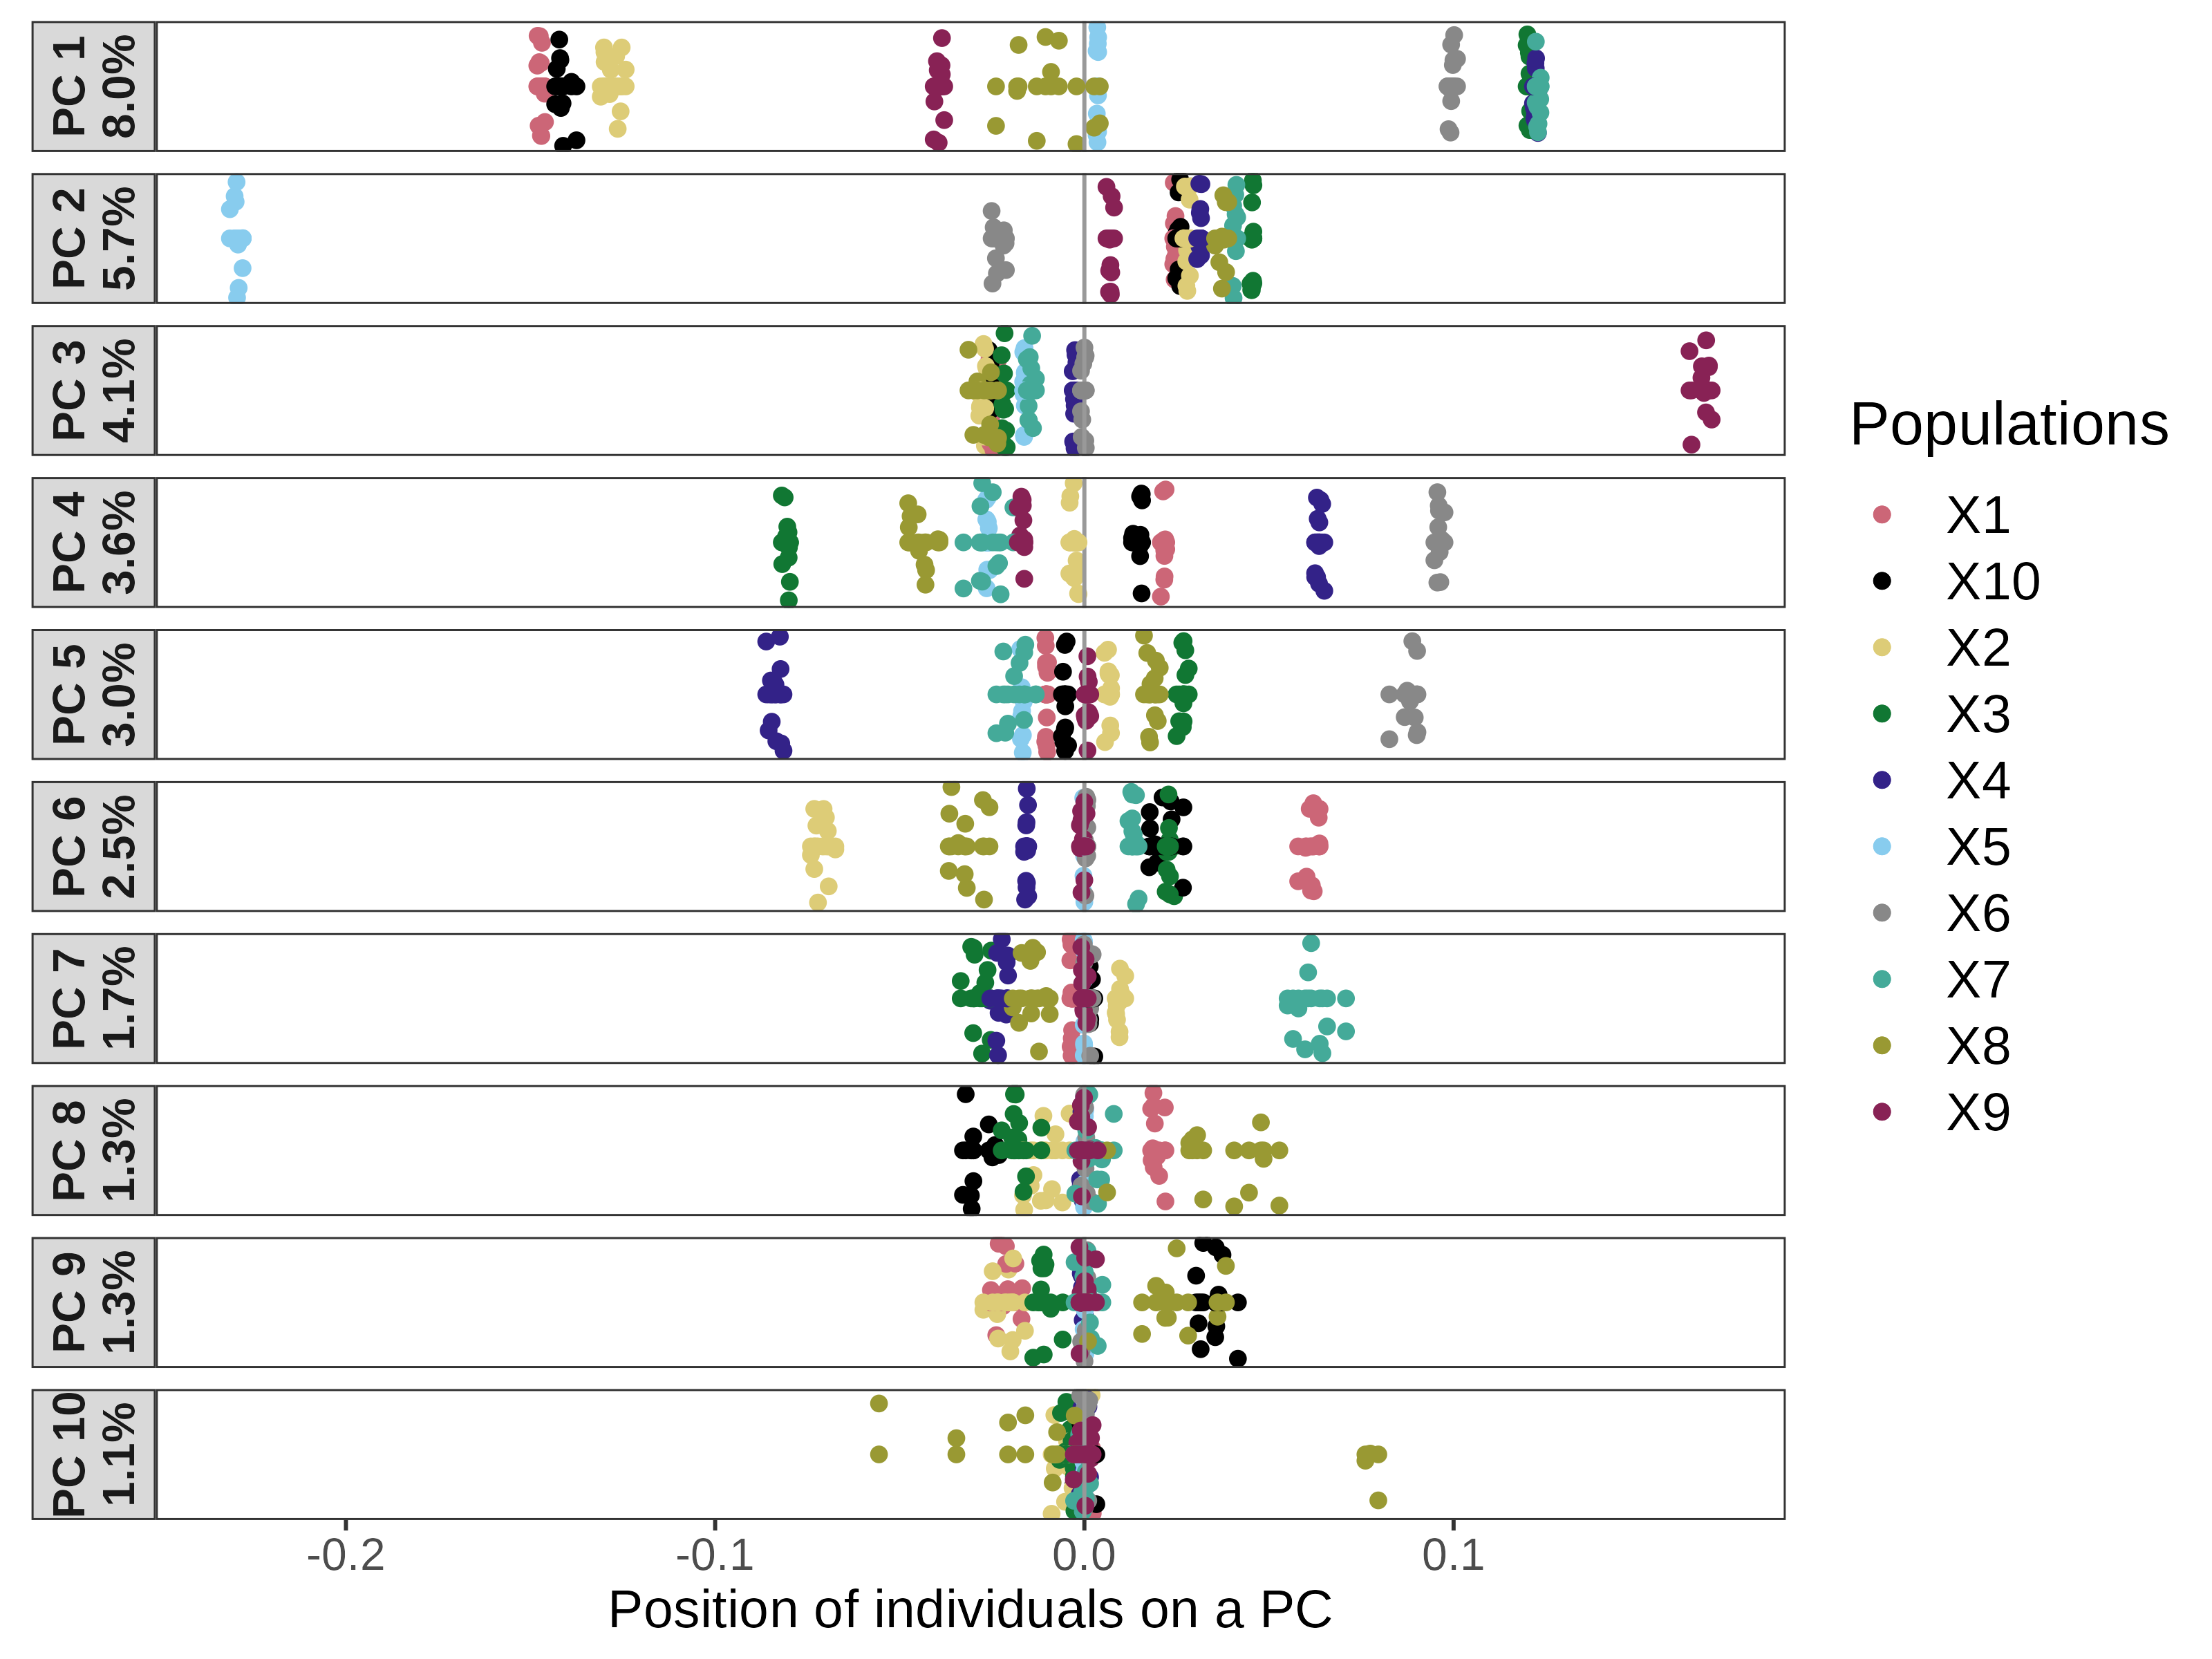
\includegraphics[width=16.5cm]{Images/Supplement/pcaplot2.png}
    \centering
    \caption{Variation in the genetic data explained with the top 10 PCs from classical PCA. Each panel shows the position of individuals on a Principal Component. Jitter is added to y-axis to show the data points clearly.}
    \label{figS1:pc_scale}
\end{figure}

\begin{figure}[ht!]
    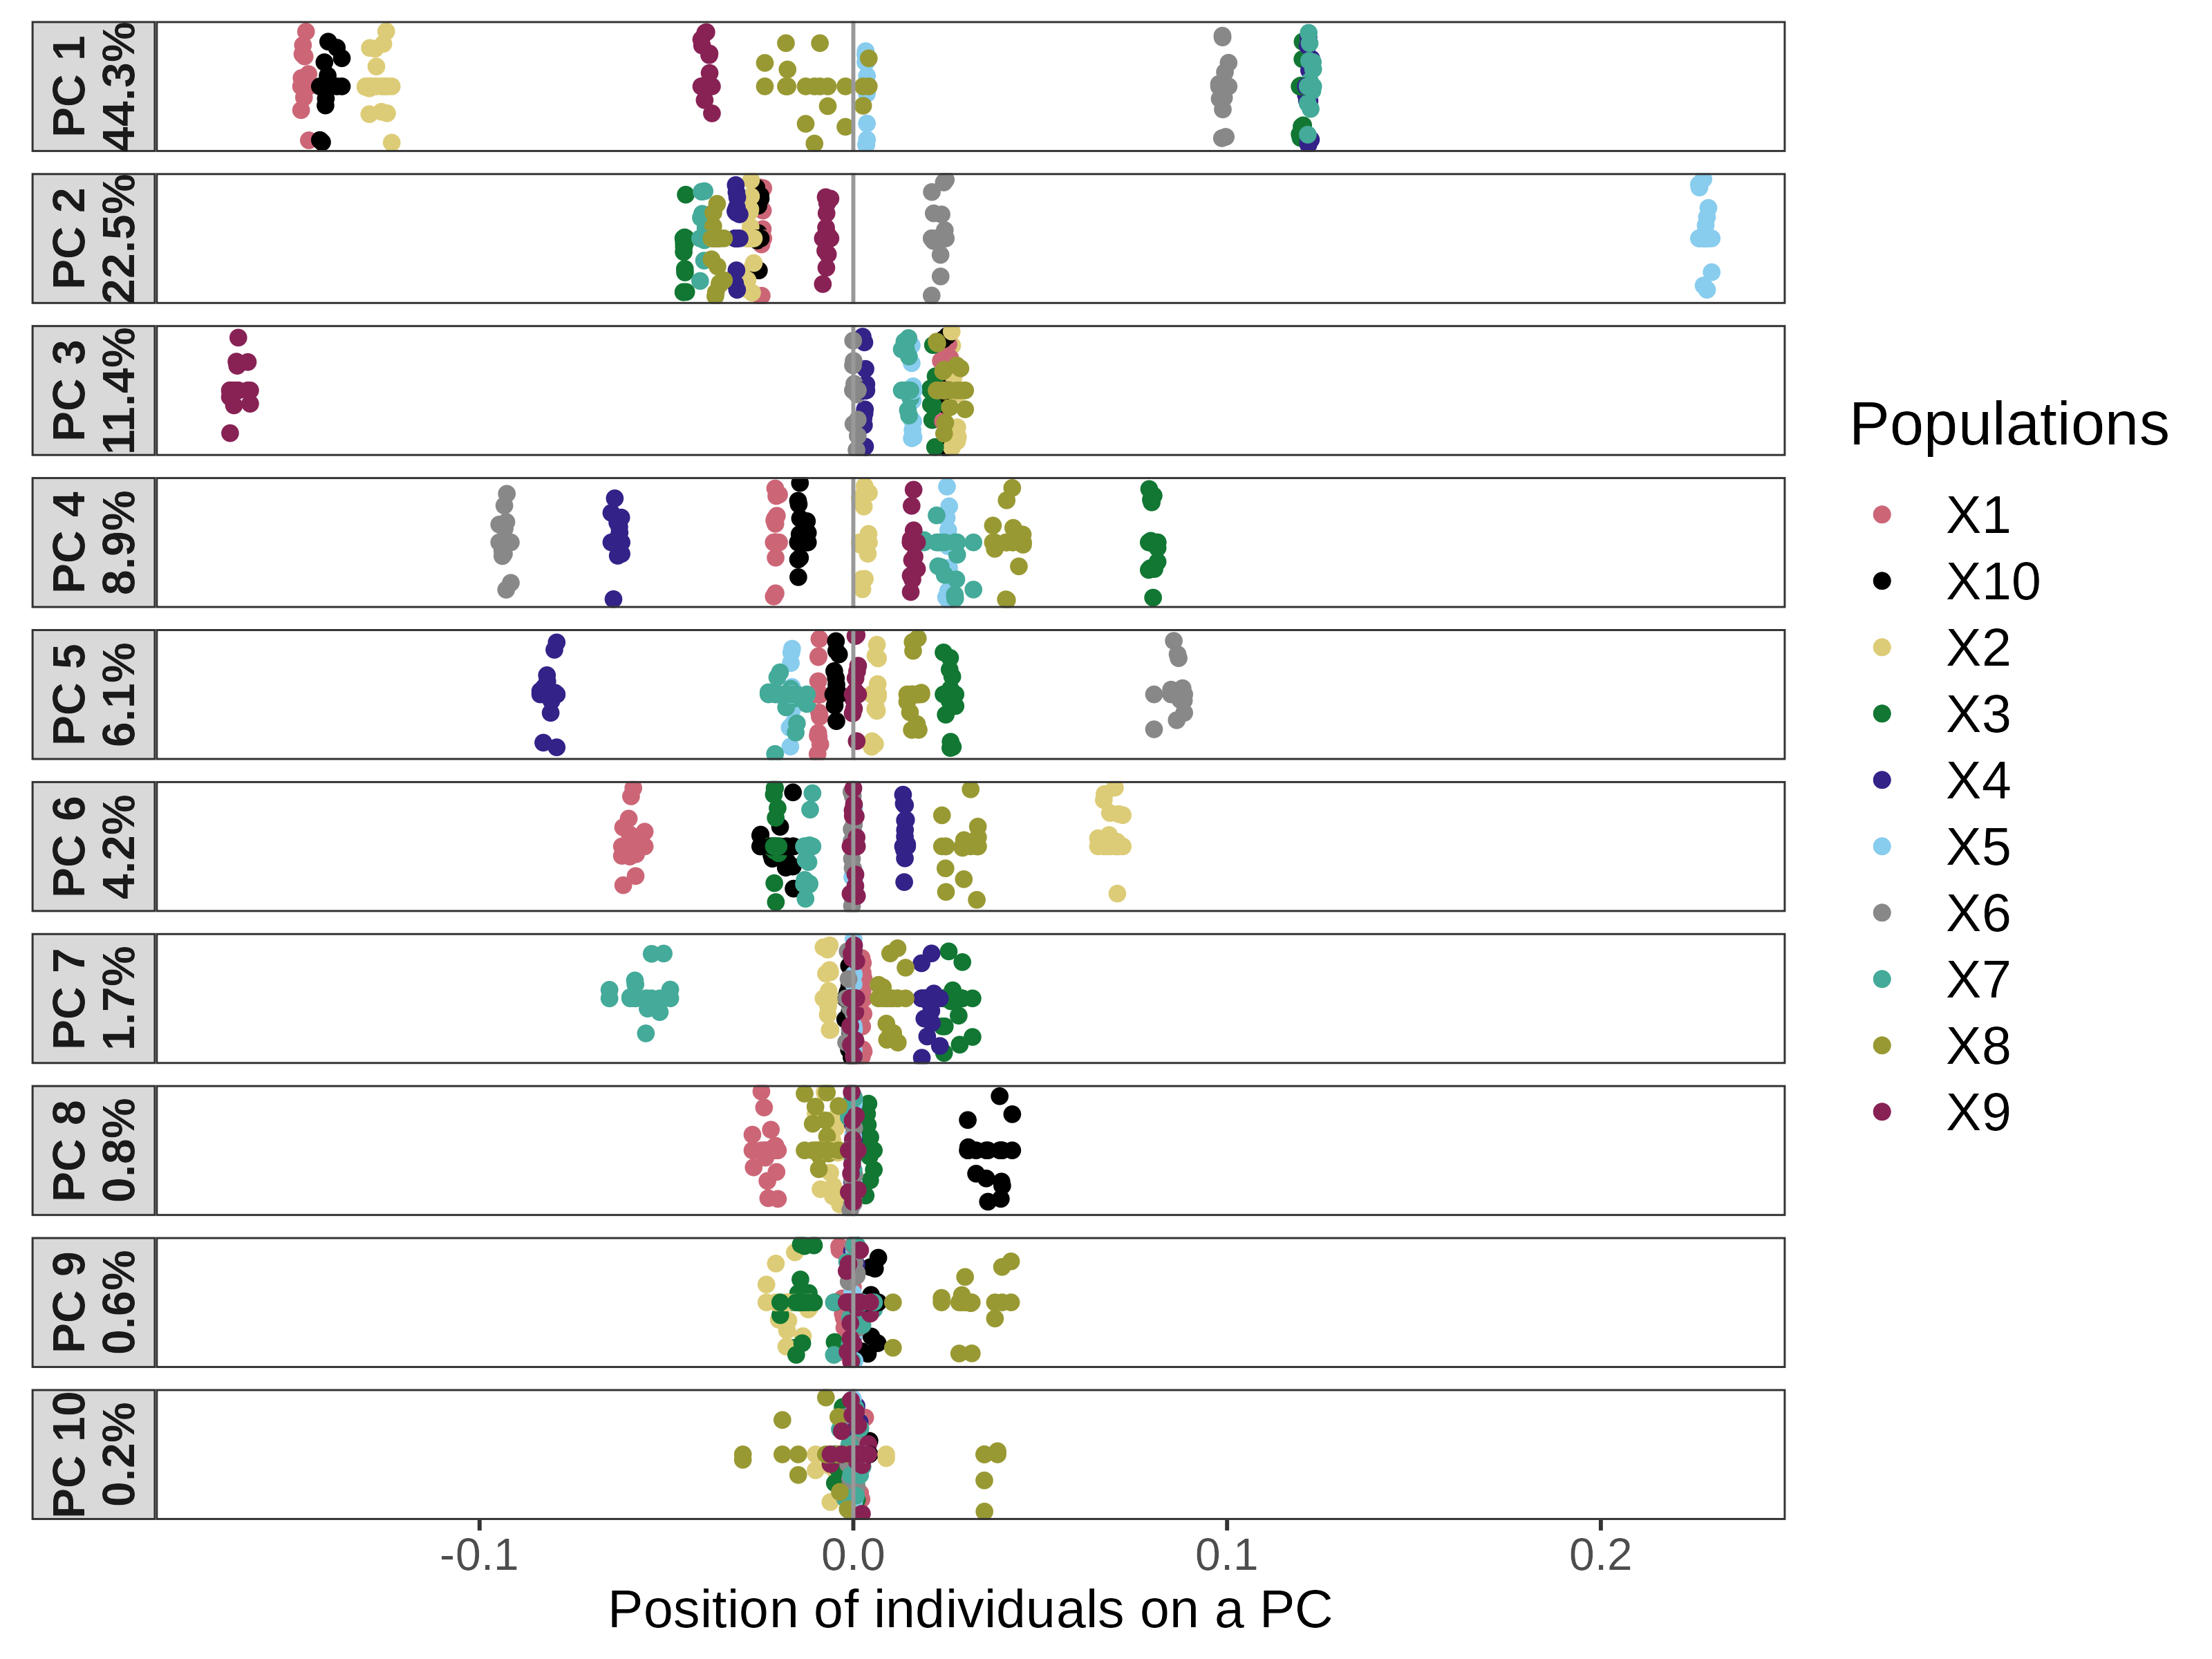
\includegraphics[width=16.5cm]{Images/Supplement/lseplot2.png}
    \centering
    \caption{Variation in the genetic data explained with the top 10 PCs from LSE. Each panel shows the position of individuals on a Principal Component. Jitter is added to y-axis to show the data points clearly.}
    \label{figS1:pc_scale}
\end{figure}


\begin{figure}[ht!]
    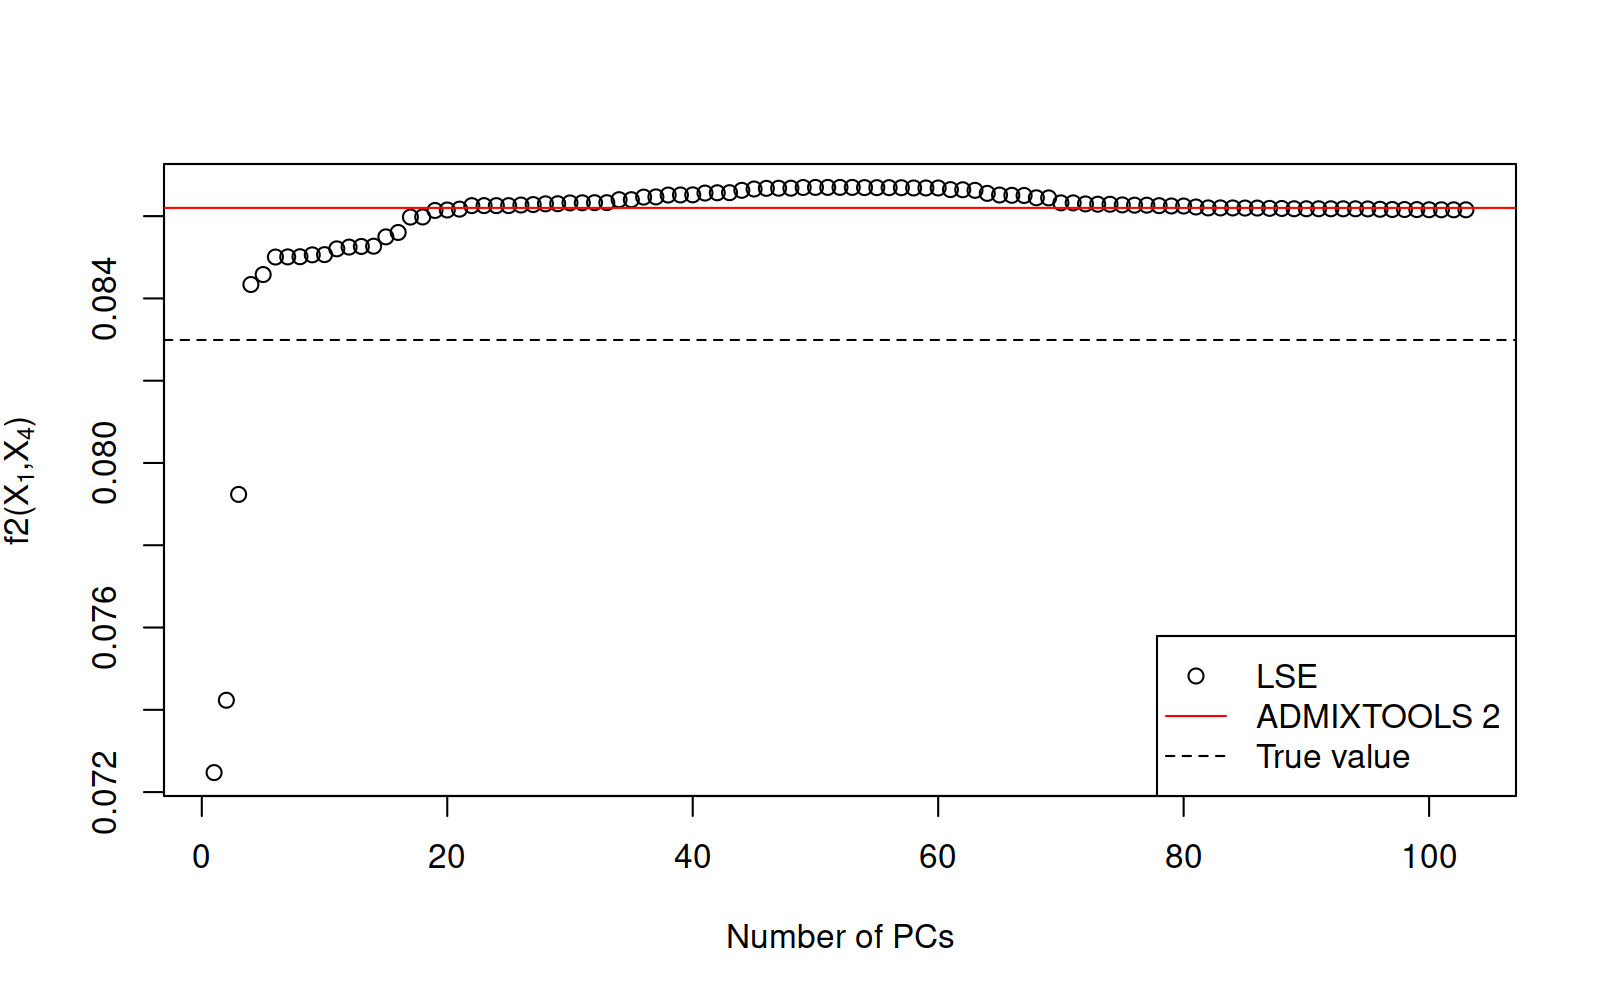
\includegraphics[width=16.5cm]{Images/Supplement/lse_admix.png}
    \centering
    \caption{$f_2(X_1,X_4)$ estimated with LSE converges to the estimate from ADMIXTOOLS 2, when all PCs are used.}
    \label{figS1:pc_scale}
\end{figure}


\begin{figure}[ht!]
    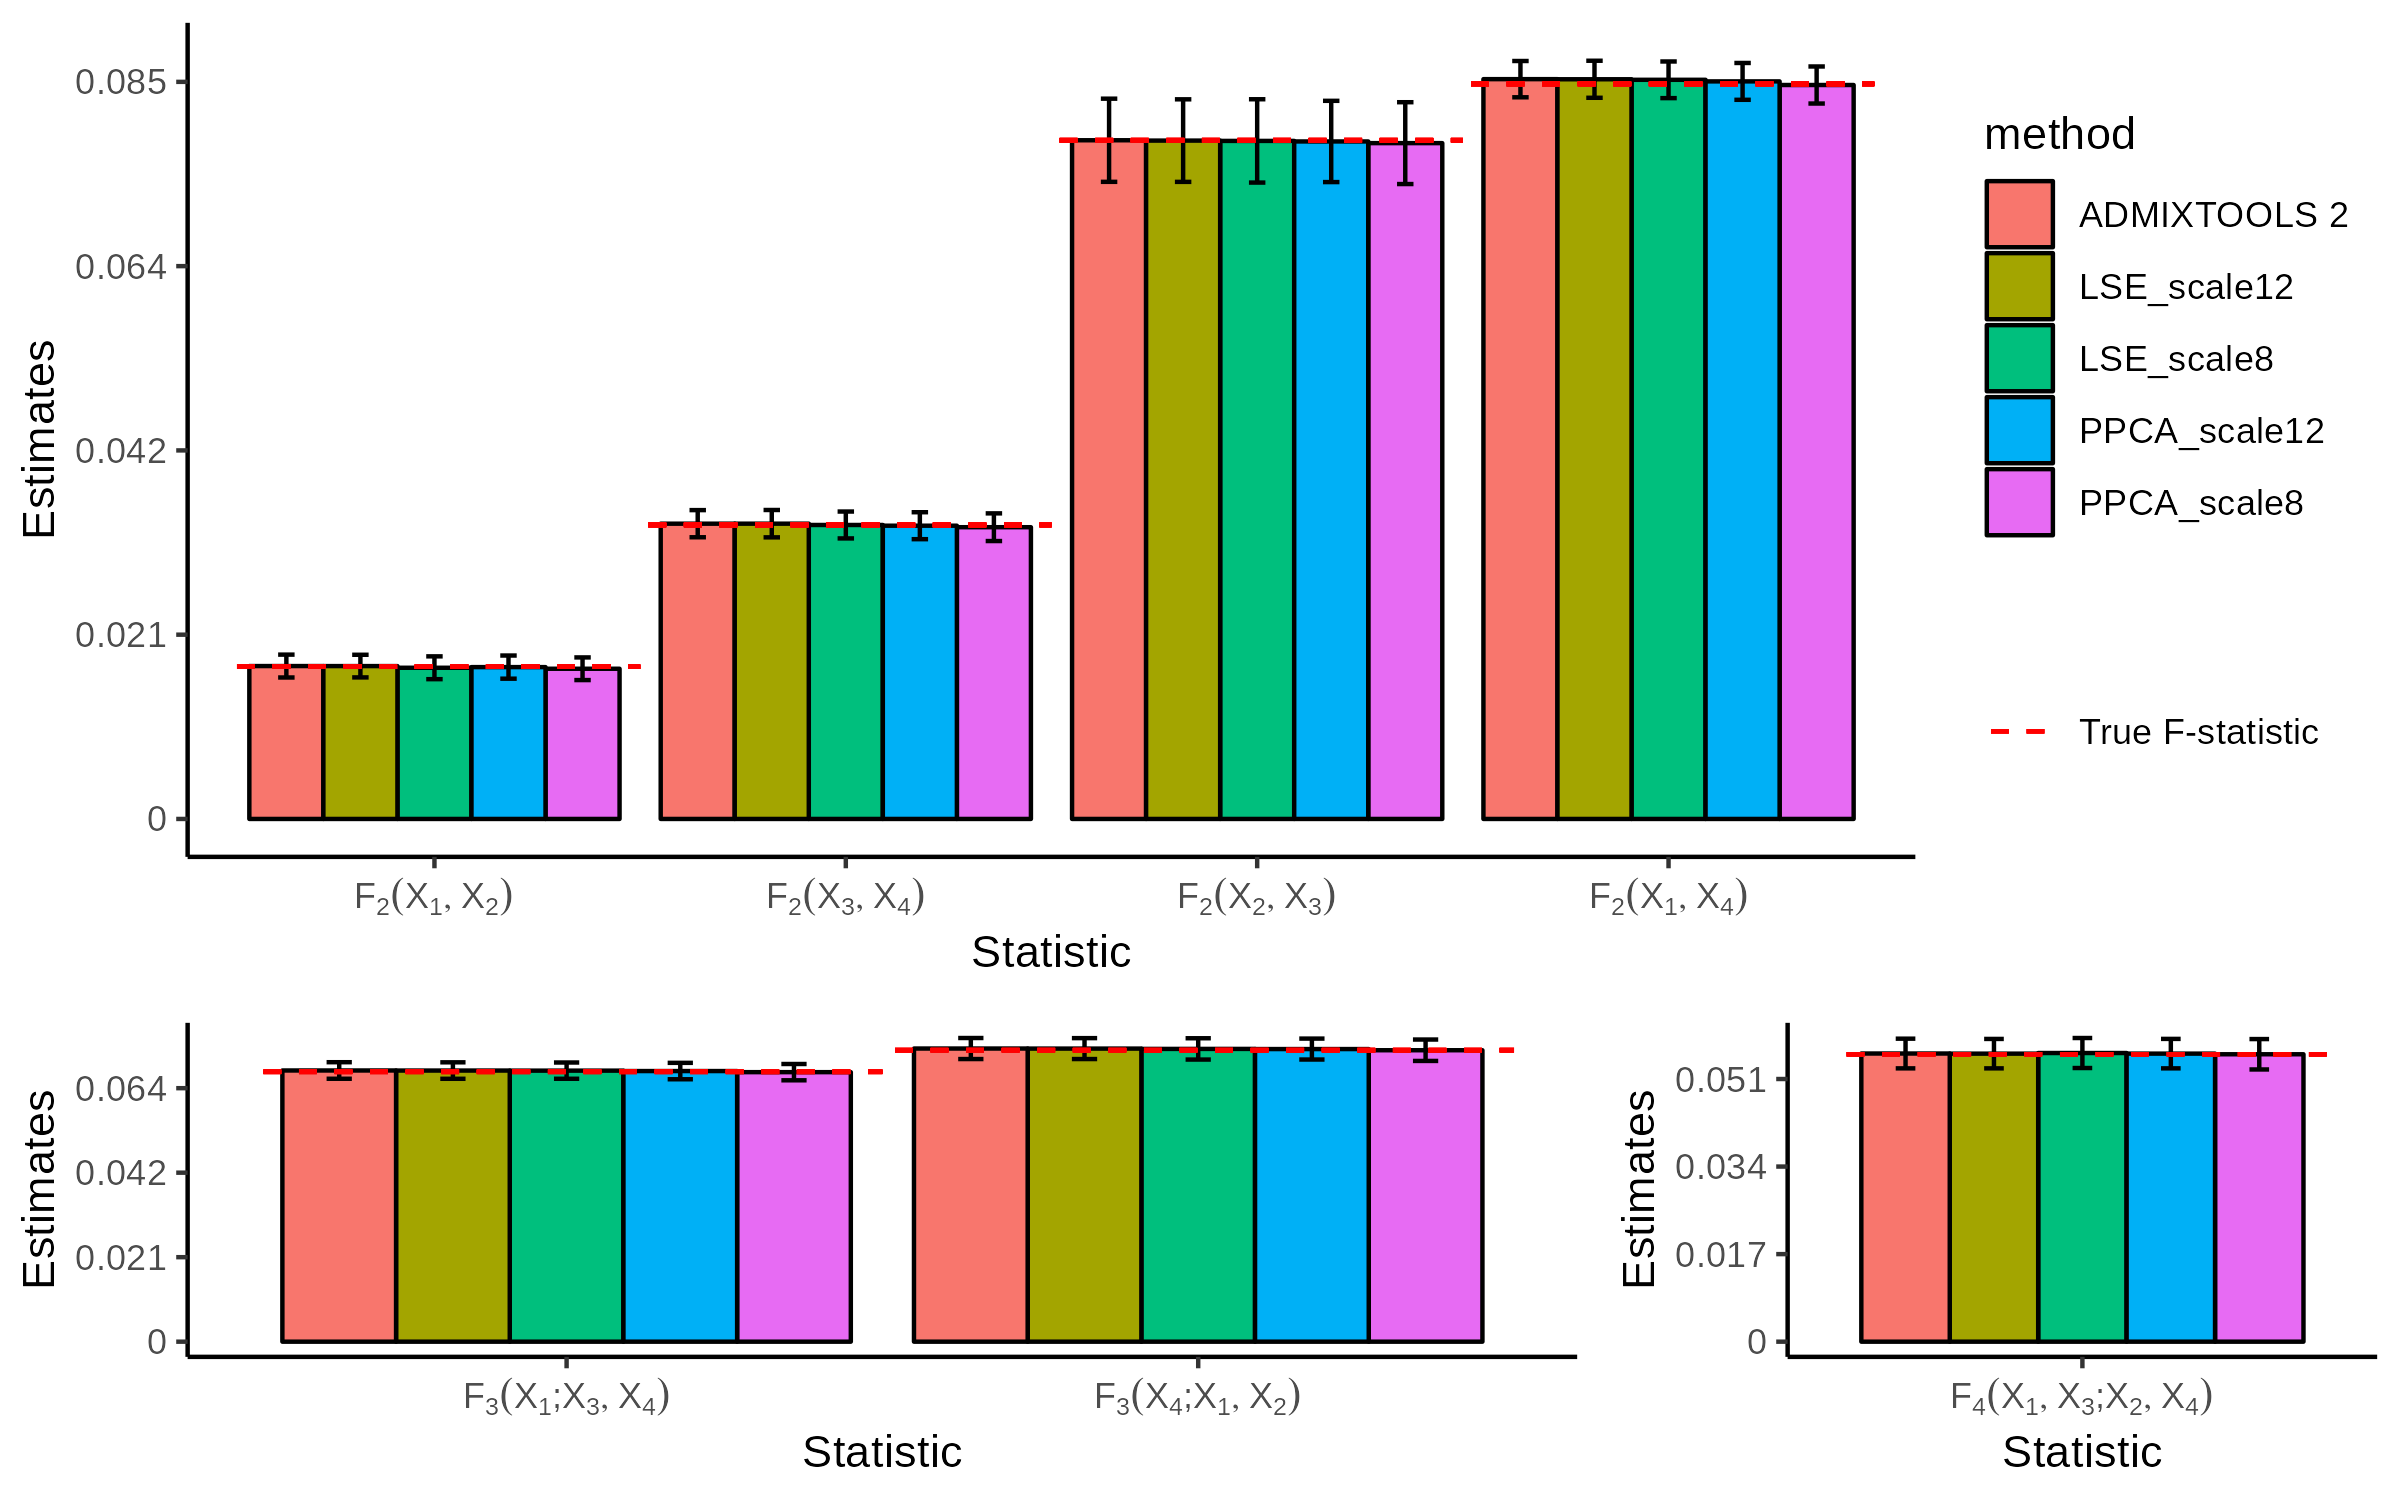
\includegraphics[width=16.5cm]{Images/Supplement/mu0.05_plot_all.png}
    \centering
    \caption{Comparison of PPCA and LSE to ADMIXTOOLS 2 using genotypes from ten individuals in each population. Top panel shows $F_2$ estimates for different populations, and the bottom left and right panels show estimates for $F_3$ and $F_4$ respectively.}
    \label{figS2:pc_scale}
\end{figure}

\begin{figure}[ht!]
    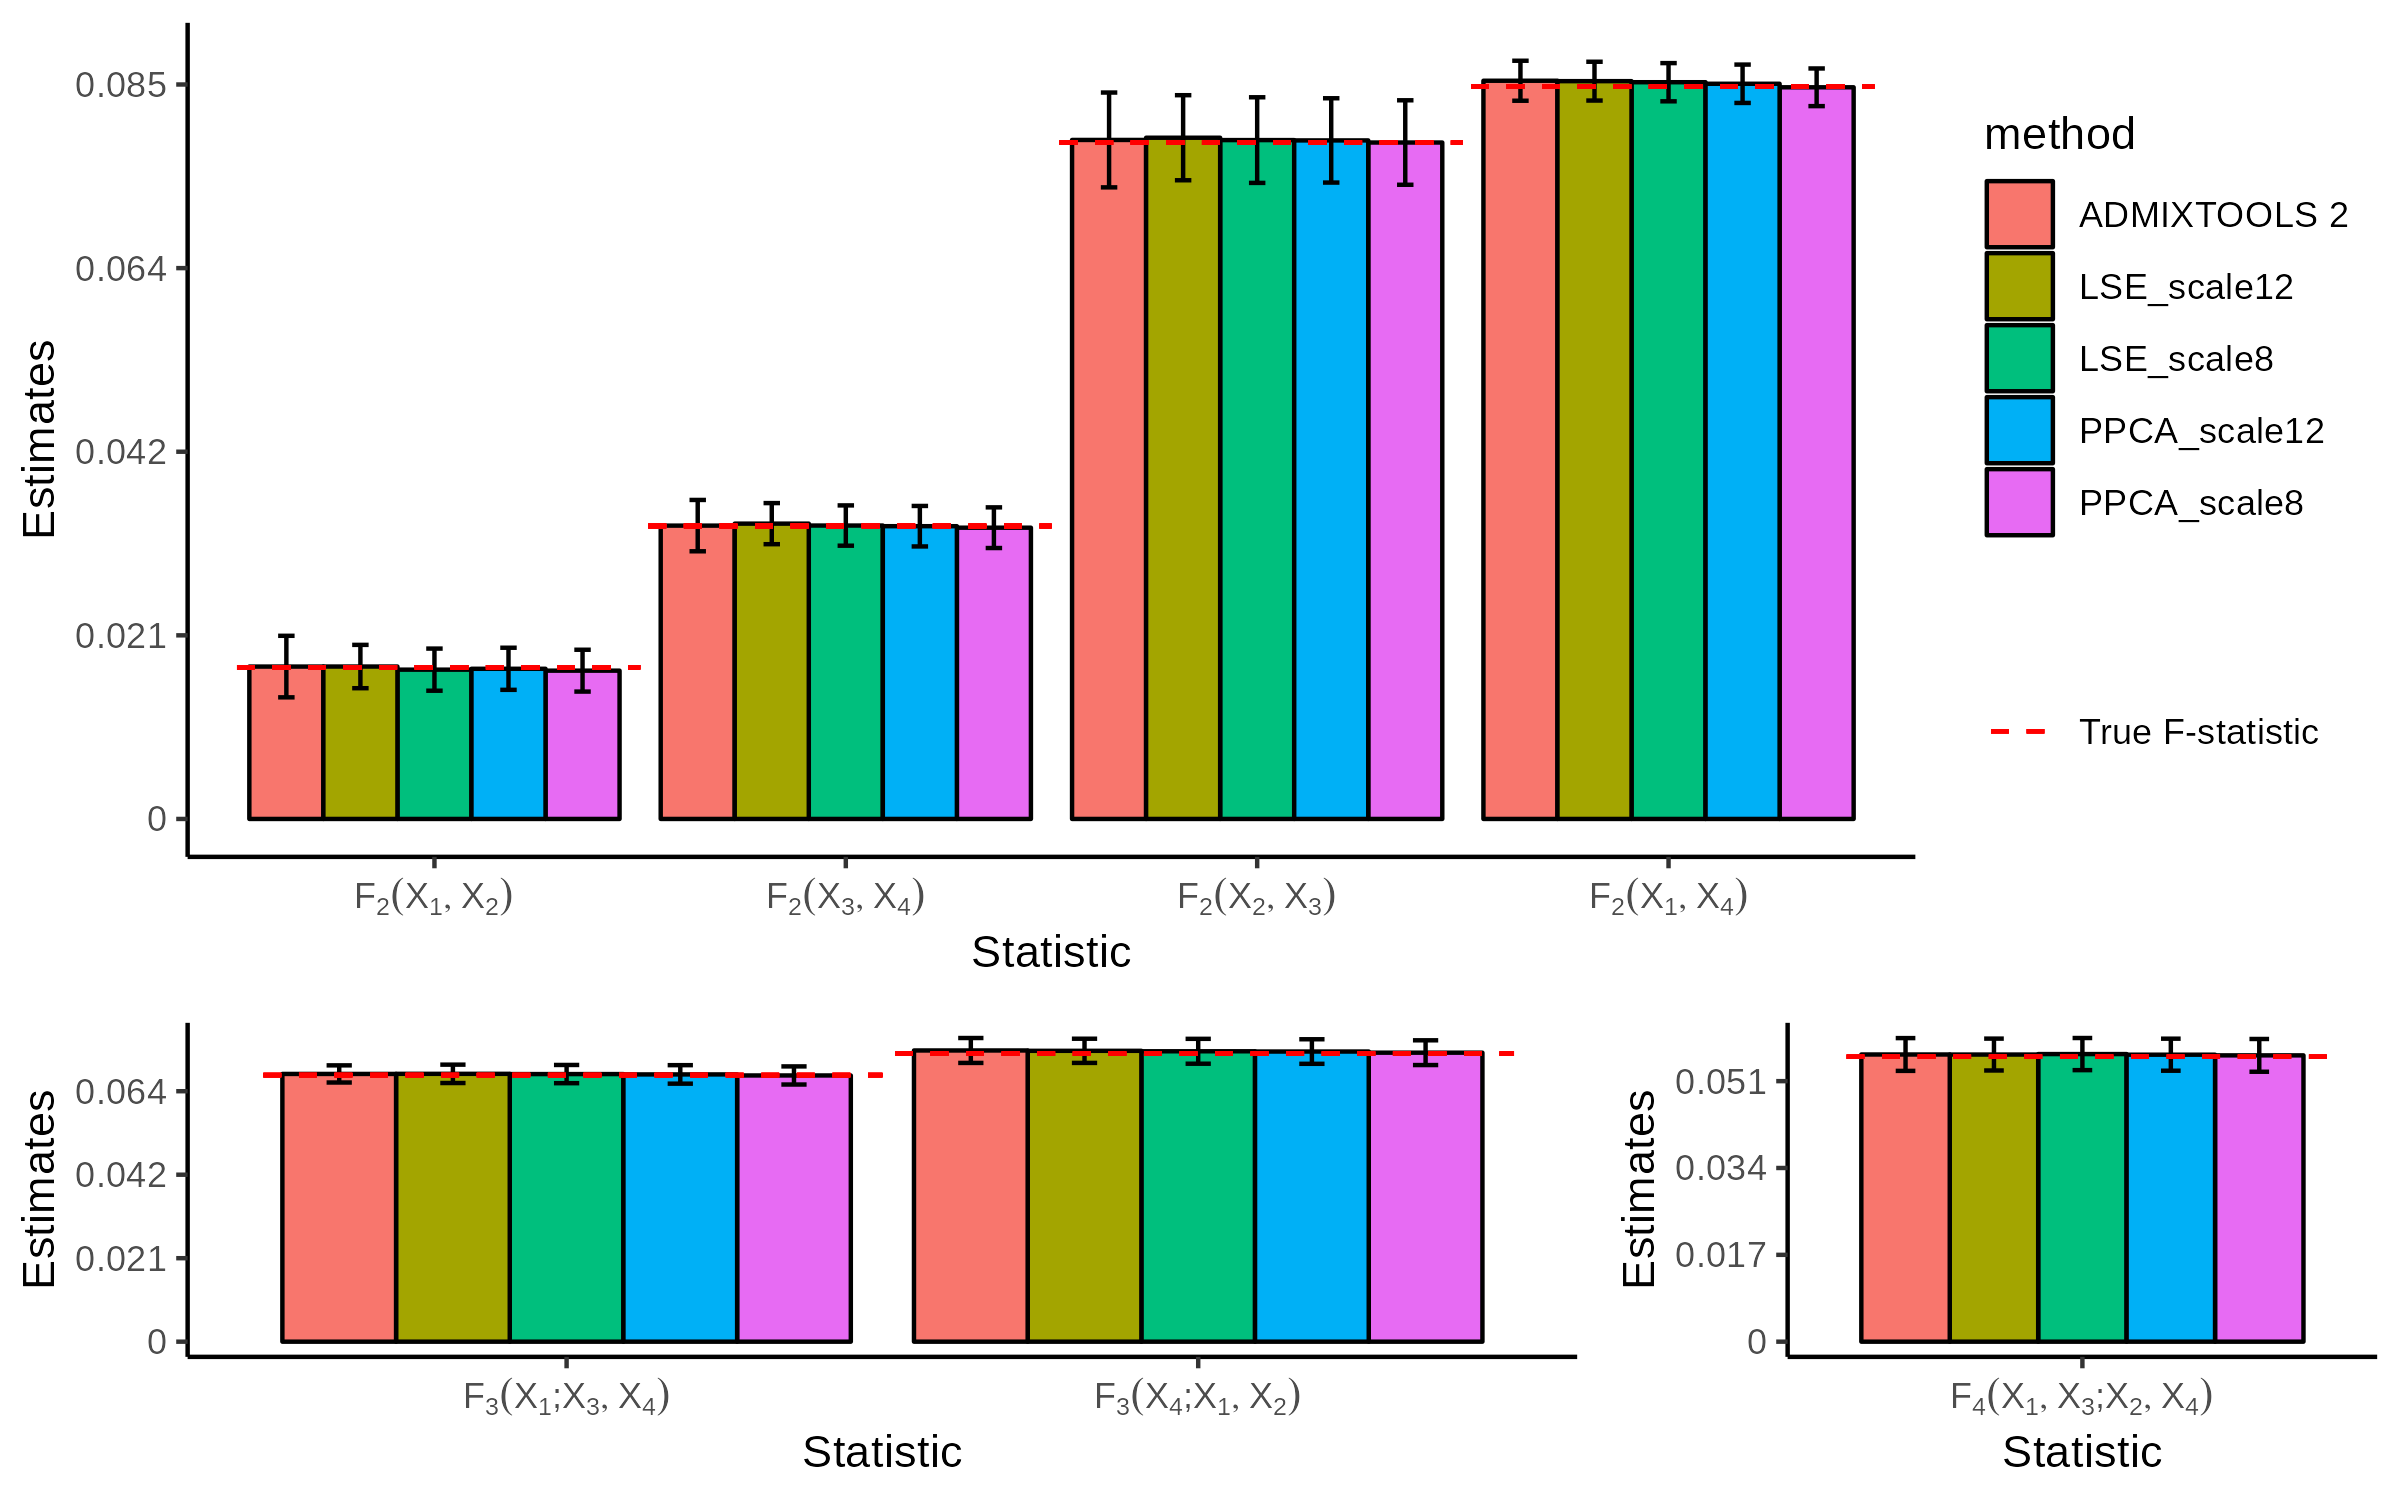
\includegraphics[width=16.5cm]{Images/Supplement/mu0.05_plot_all_1ind.png}
    \centering
    \caption{Comparison of PPCA and LSE to ADMIXTOOLS 2 using genotypes from one individual from each population. Top panel shows $F_2$ estimates for different individuals, and the bottom left and right panels show estimates for $F_3$ and $F_4$ respectively.}
    \label{figS2:pc_scale}
\end{figure}

\begin{figure}[ht!]
    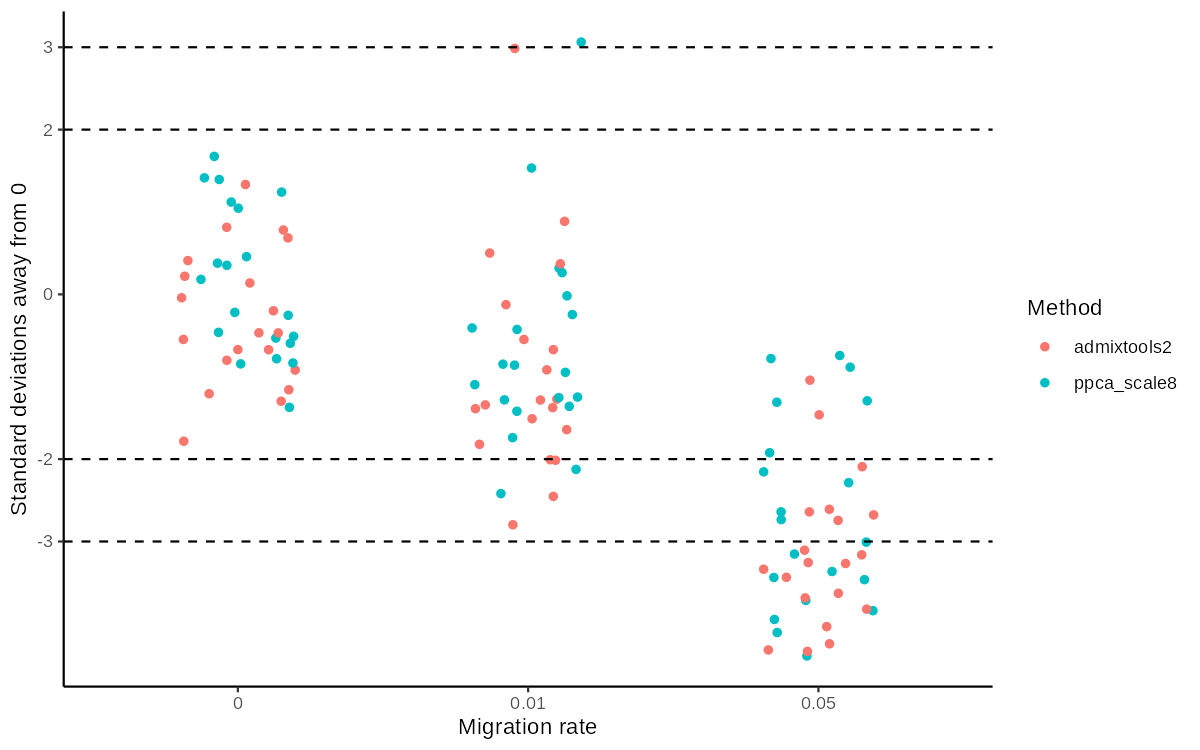
\includegraphics[width=16.5cm]{Images/Supplement/hypothesis_test_comparison.png}
    \centering
    \caption{Test for admixture with F4 statistic. We compare ADMIXTOOLS 2 (orange)to PPCA-based-framework (blue). Horizontal dashed lines denote 2 and 3 standard deviations from the mean.} 
    \label{figS2:pc_scale}
\end{figure}

\begin{figure}[ht!]
    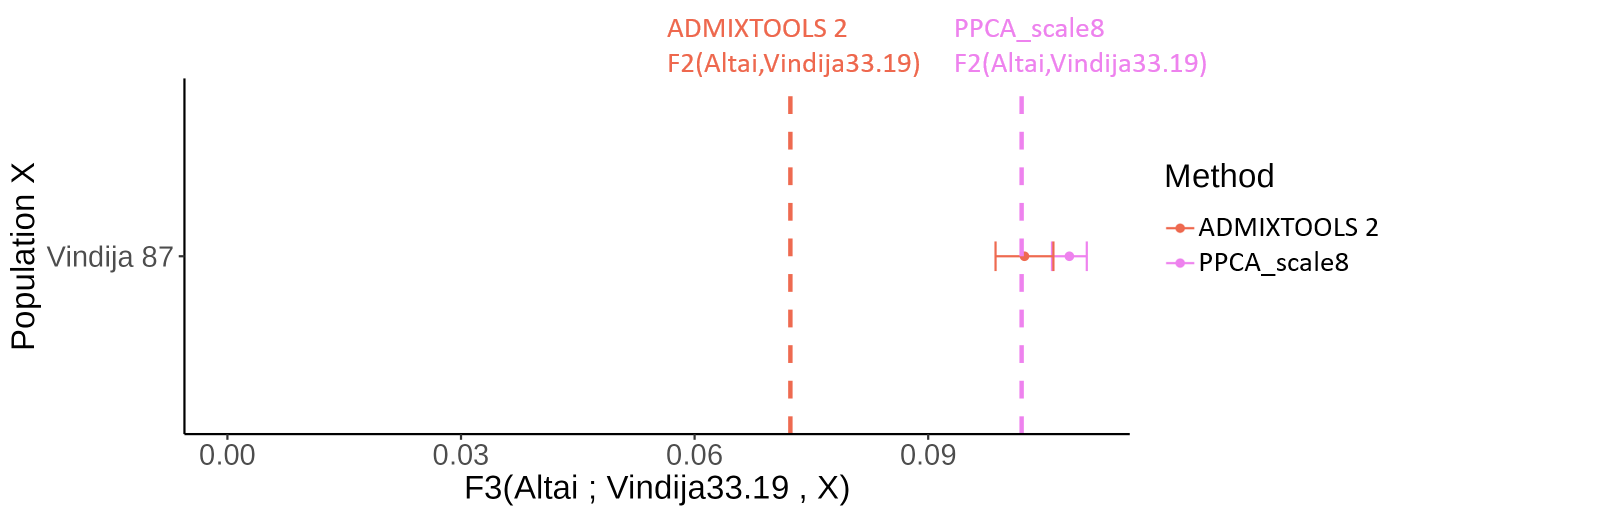
\includegraphics[width=16.5cm]{Images/Supplement/f2_f3_corr.png}
    \centering
    \caption{Comparison of f3(Altai ; Vindija33.19, X) with f2(Altai, Vindija33.19) (shown in dashed lines) estimated with ADMIXTOOLS 2 and PPCA with 8 PCs. The red and purple arrows show the distance between the f2 and f3 statistics estimated from ADMIXTOOLS 2 and PPCA respectively.} 
    \label{figS2:pc_scale}
\end{figure}



\end{document}